\section{Architecture 102}

%\subsection{}

%\subsubsection{}

\textbf{Architectures:}
\begin{itemize}
	\item The art or practice of \textbf{designing} and \textbf{building} structure and especially habitable ones.
	\item A unifying or coherent \textbf{from} or \textbf{structure}
\end{itemize}

\textbf{Foundation for the study of Software Architecture / L. Wolf, 1992}

Software architecure principles can be \textbf{inherited} by appealing to several well-established architectural disciplines.

While the subject matter for the two is quite different, there are a number of intresting \textbf{architectural points} in building architecture that are suggestive for software architecture
\begin{itemize}
	\item multimple \textbf{views}
	\item architectural \textbf{styles}
	item style and \textbf{materials}
+\end{itemize}

\subsection{Preliminary Concept}

\textbf{Never take anything for granted}

\subsubsection{Apache Kafka and Pub/Sub}

\begin{itemize}
	\item Kafka is a \textbf{distributed system} consisting of servers and clients that communicate via a high-performance TCP network protocol.
	\item Kafka combines three key capabilities so tou can implement your use cases for \textbf{event streaming end-to-end}
	\begin{itemize}
		\item To \textbf{To publish (write} and \textbf{subscribe to} (read) streams of events, including continuous import/export of your data from other system
		\item To \textbf{store} streams of events durably and reliably for as long as you want
		\item To \textbf{process} streams of events as they occur or retrospectively
	\end{itemize}
	\item An \textbf{event} records the fact that "something happened" in the world or in your business [e.g., a user posts a tweet]
	\item \textbf{Producers} are those client applications that publish (write) events to Kafka, and \textbf{consumers} are those that subscribe to (read and process) these events. In Kafka, \textbf{producers and consumers are fully decoupled and agnostic of each other}, which is a key design element to achieve the high scalability that Kafka is known for.
	\item Events are organized and durably stored in \textbf{topics}. Very simplified, a topic is similar to a folder in a filesystem, and the events are the files in that folder. Another way to see it, the \textbf{topic is like an INDEX} on a SQL table.
\end{itemize}

\subsubsection{Extract Transform Load – ETL (*)}

\begin{itemize}
	\item In computing, extract, transform, load (ETL) is the general procedure of \textbf{copying data from one or more sources into a destination system}
	\begin{itemize}
		\item Data extraction involves \textbf{extracting data from homogeneous or heterogeneous} sources
		\item Data transformation processes data by \textbf{data cleaning and transforming them into a proper storage format/structure} for the purposes of querying and analysis
		\item Data loading describes \textbf{the insertion of data into the final target database} such as an operational data store, a data mart, data lake or a data warehouse
	\end{itemize}
	\item ETL can be used:
	\begin{itemize}
		\item to increase data quality and consistency
		\item to normalize data
		\item to apply simple/complex logics such as id to string conversion through a lookup table
		\item to prepare data for a presentation layer
	\end{itemize}
	\item ETL can be one-shot or incremental
\end{itemize}

\subsubsection{Object Storage Model}
\begin{itemize}
	\item Object storage is a \textbf{computer data storage architecture} that manages data asobjects. It is opposed to other storage architectures like file systems or block storage
	\item Each object typically contains \textbf{data, contextual information} (metadata), and \textbf{technical information} (header)
	\item It is based on a \textbf{shared naming convention}, which generates a unique id for each object, and a shared \textbf{serialization strategy} (e.g., json)
	\item It allows to \textbf{distribute data} over several nodes
	\item Object storage was created to allow \textbf{retention} of massive amounts of unstructured data
\end{itemize}

\subsubsection{Data Lake}
\begin{itemize}
	\item Models you can build using data cannot \textbf{be known a priori}: if some pieces ofinformation are not saved when produced (e.g., under sampling a sensor), they \textbf{could not be re-acquired later}
	\item \textbf{Legacy Systems} integration is pretty complex and expensive: once a legacy system is integrated, there is no reason not to get all available information
	\item Other Data Architectures have problems dealing with \textbf{heterogeneous data} or data which format and content can \textbf{change over time}
	\item Data Lakes is based on \textbf{four pillars}:
	\begin{itemize}
		\item Unprocessed data (only serialized in objects)
		\item Data saved forever
		\item Good reading/writing performances
		\item Schema available on read
	\end{itemize}
\end{itemize}

\subsubsection{Concrete and Abstract Classes}
\begin{itemize}
	\item Concrete Class
	\begin{itemize}
		\item A concrete class is a class that can be instantiated
	\end{itemize}
	\item Abstract Class
	\begin{itemize}
		\item Cannot be instatied
		\item Contains Abstract Methods
		\item Can contain concrete methods
		\item Specifies virual methods via signatures that are to be implemented
		\item Before a class derived from an abstract class can be instantiated, all abstract methods of its parent classes must be implemented
	\end{itemize}
\end{itemize}

\subsubsection{Lock-in}
\begin{itemize}
	\item Vendor lock-in makes \textbf{a customer dependent on a vendor} for products and
services
	\item A supplier \textbf{successfully locks in} a customer when:
	\begin{itemize}
		\item \textbf{the cost of changing} supplier is higher that the cost of keeping it
		\item without that cost, other \textbf{suppliers can outperform} the actual supplier
	\end{itemize}
	\item An Enterprise Architecture can protect the company from Vendor lock-in
	\item Another kind of lock-in is the so called \textbf{knowledge lock-in}: this kind of lock-in happens when the \textbf{cost of knowledge transfer} is higher than the benefit to dismiss a person/team. Again, a Software Architecture can \textbf{mitigate this risk}
\end{itemize}

\subsection{Software Architecture Pillars}

\subsubsection{8 reasons why}

\begin{center}
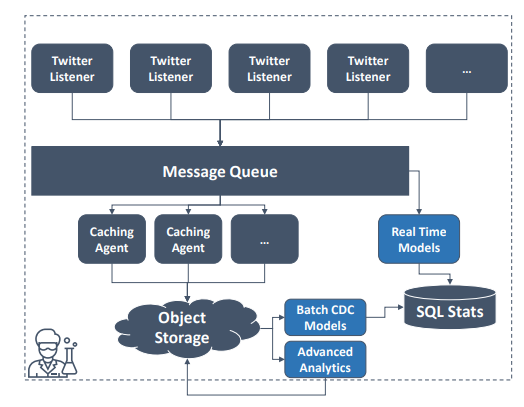
\includegraphics[scale=0.7]{13-architecture-pillars-on-BOC-app}
\end{center}

\textbf{Bully Operation Center}
\begin{itemize}
	\item A WebApp supports \textbf{a group of Analysts} to spot \textbf{aggressive users}
	\item Natural Language Processing is used to \textbf{classify} each tweets
	\item When the \textbf{number of aggressive tweets} done by a given user go beyond a given threshold, this user is surfaced to an Analyst \textbf{who can decide to ban} it
	\item When a user is classified by the Analyst as bully, \textbf{the number of mbullied users} is computed as the number of users after a bully user comment stop to use tweeter
\end{itemize}

\subsubsection{Software Architecture Pillars}
\begin{enumerate}
	\item Being the framework for satisfying requirements
	\item Being the technical basis for design 
	\item Being the managerial basis for cost estimation and process management
	\item Enabling component reuse
	\item Focus on centralization
	\item Enhancing productivity and security
	\item Enabling enterprise systems integration (Enterprise Application Integration)
	\item Allowing a tidy scalability
	\item Controlling software processes execution
	\item Avoiding handover and people lock-in
\end{enumerate}

\subsubsection{Being the framework for satisfying requirements}
\begin{center}
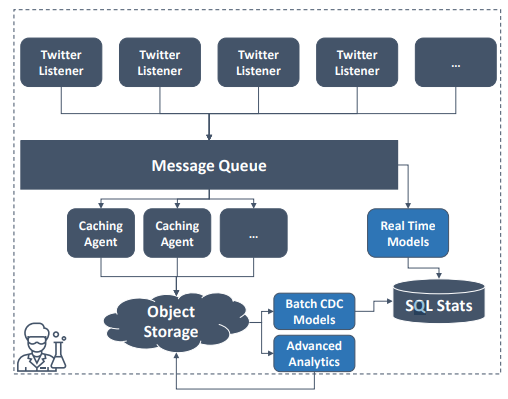
\includegraphics[scale=0.7]{14-being-the-framework-for-satisfying-requirements}
\end{center}
\begin{itemize}
	\item Functional Requirement
	\begin{itemize}
		\item Am I able to spot aggressive users?
		\item Will the Analyst have all the needed information to decide to ban a user?

	\end{itemize}
	\item Technical Requirement
	\begin{itemize}
		\item Am I able to process all the tweets in time?
		\item Am I able to check in the history bullied users?
	\end{itemize}
	\item Security Requirement
	\begin{itemize}
		\item Is it compliance with GDPR (data privacy rules)?
	\end{itemize}
\end{itemize}

\subsubsection{Being the technical basis for design}
\begin{center}
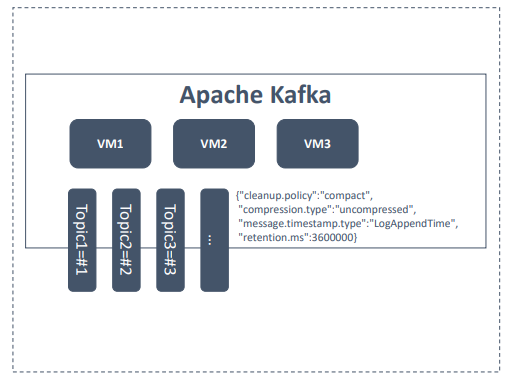
\includegraphics[scale=0.5]{15-being-the-technical-basis-for-design}
\end{center}

Modularization and detailed interfaces of the design elements, their algorithms and procedures, and the data types needed to support the architecture and to satisfy the requirements

\subsubsection{Being the managerial basis for cost estimation and process
management}
\begin{center}
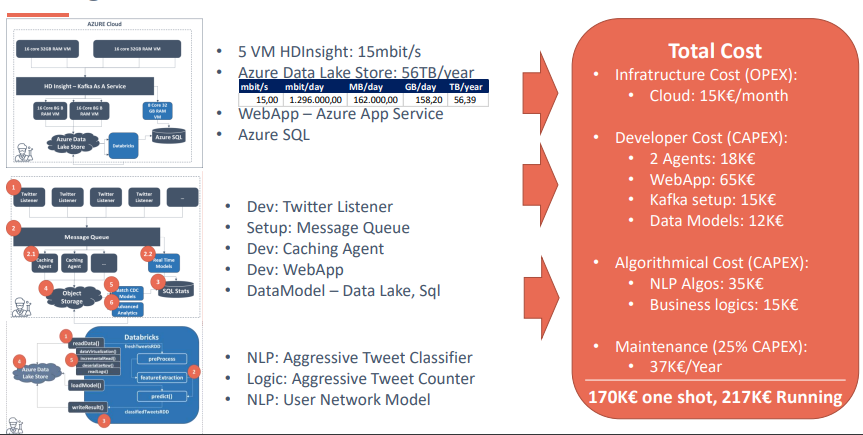
\includegraphics[scale=0.5]{16-being-the-managerial-basis-for-cost-estimation-and-process}
\end{center}

\subsubsection{Enabling component reuse}
\begin{center}
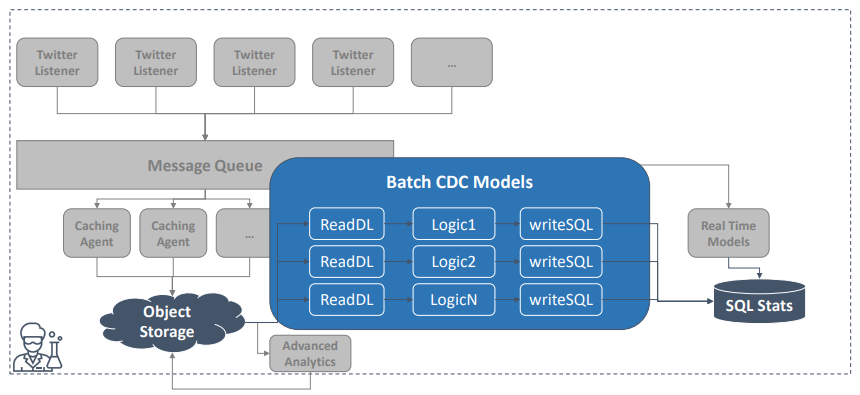
\includegraphics[scale=0.5]{17-enabling-component-reuse}
\end{center}

\subsubsection{Focus on centralization}
\begin{center}
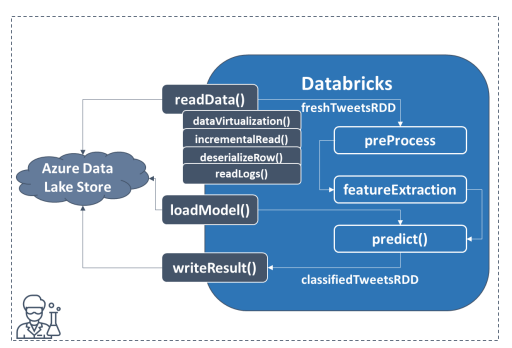
\includegraphics[scale=0.7]{18-focus-on-centralization}
\end{center}

\begin{itemize}
	\item Azure Data Lake Store in our Architecture is the Single Source of Truth
	\item Data are Centralized there
\end{itemize}

\subsubsection{Enhancing productivity and security}
\begin{center}
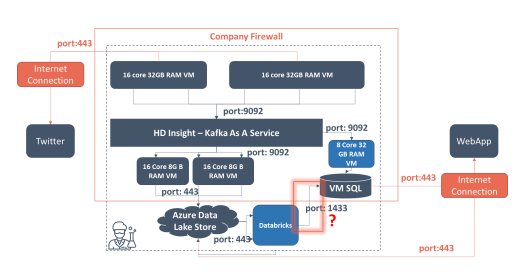
\includegraphics[scale=0.9]{19-enhancing-productivity-and-security}
\end{center}

\begin{itemize}
	\item We know exactly which ports we need to open
	\item We can build a gateway to access SQL data from WebApp to avoid SQL Injection (access is centralized there)
	\item We can build the component to hide Data Lake and enforce ACL Rules
\end{itemize}

\subsection{Design patterns}
Design paterns are\textbf{formalized best practices} found to solve \textbf{common problems}

\subsubsection{Hundreds of Design Pattern}
\begin{center}
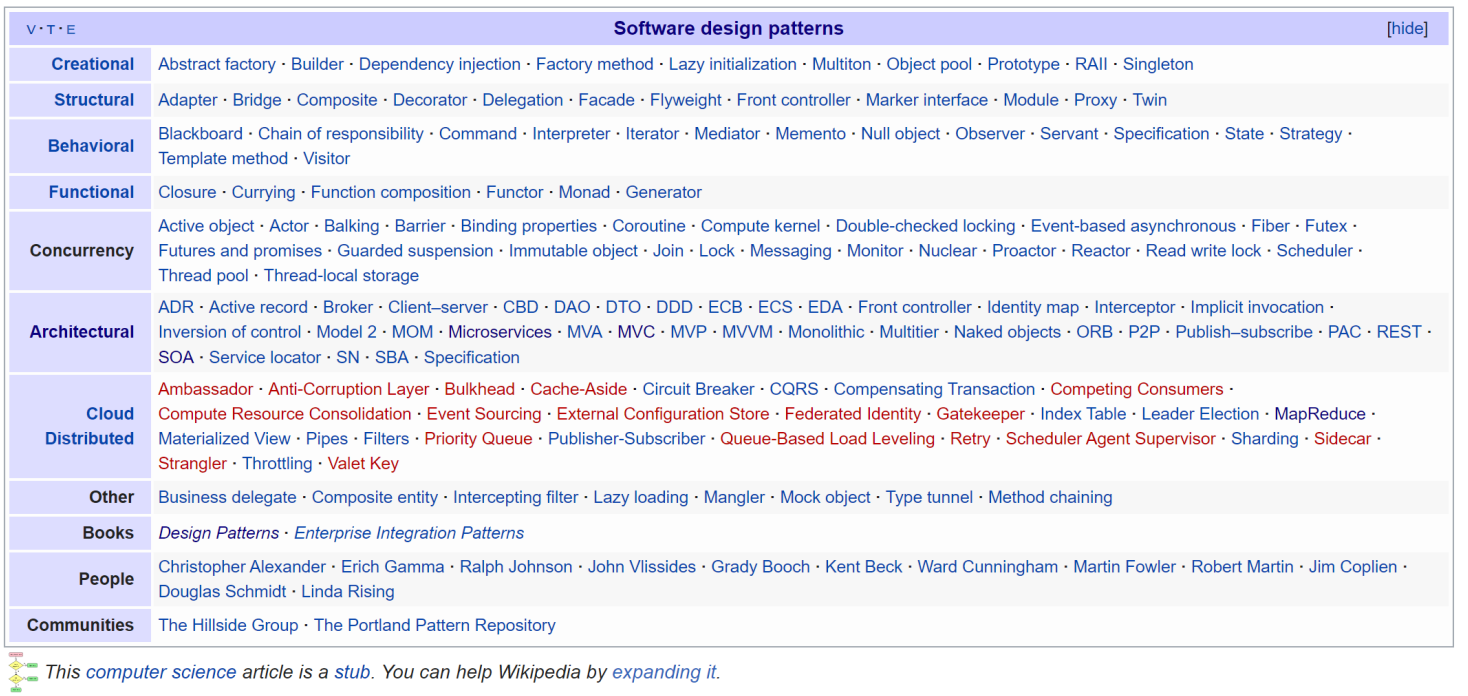
\includegraphics[scale=0.35]{20-hundreds-of-degisn-pattern}
\end{center}

\subsubsection{The 23 Classical Patterns by Type}
\begin{center}
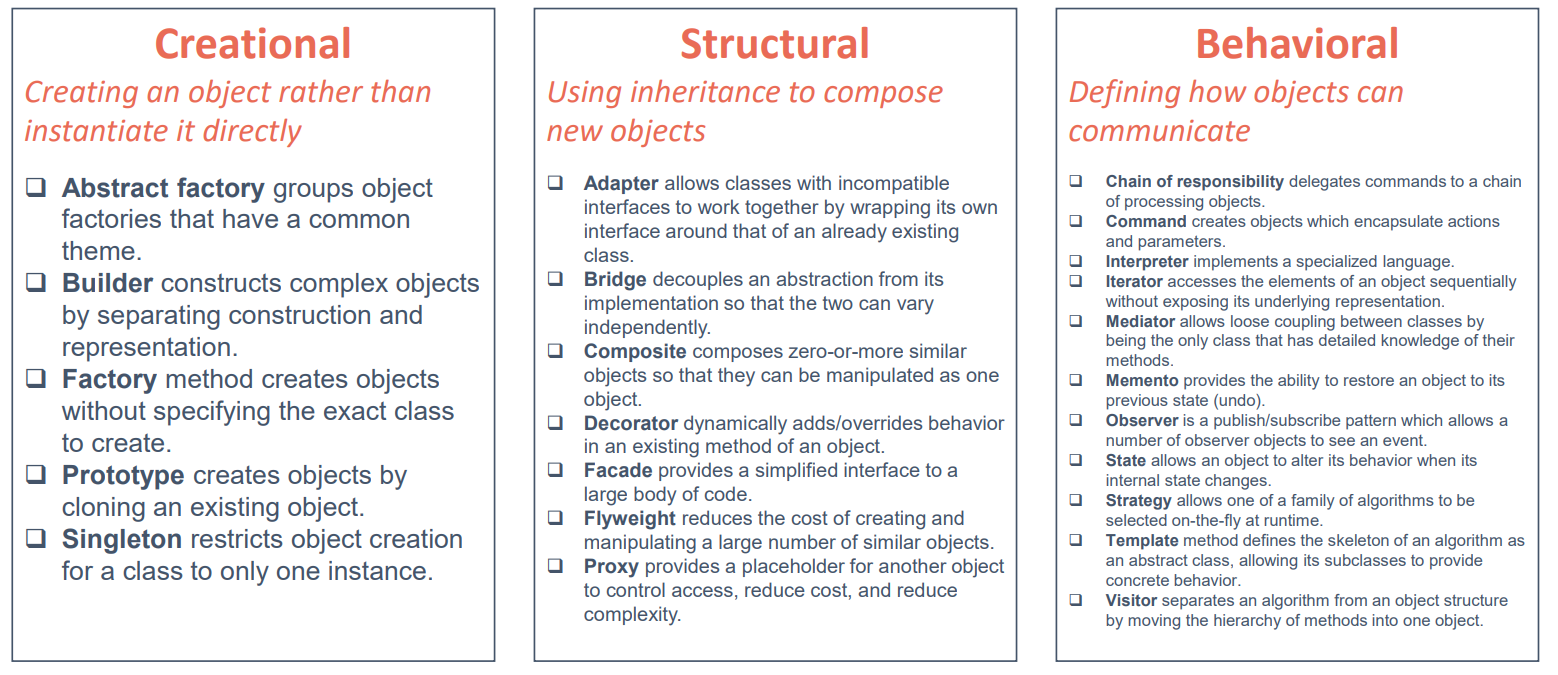
\includegraphics[scale=0.3]{21-the-23-classical-pattern-by-type}
\end{center}

\subsubsection{The Adapter Pattern (Wrapper)}

Problem - Vendor Lock-In

\begin{center}
%\includegraphics[scale=0.35]{}
\end{center}

\begin{itemize}
	\item
	\item
\end{itemize}

\subsubsection{A step back: on the origin of the system}
Problem - Operational System are always under pressure

\textbf{Transactional/Operational System}
\begin{itemize}
	\item Critical System used  to support the company daily activities
	\item Any process risking to impact on their performance should be avoided
\end{itemize}

\textbf{Informative/Analytical System}
\begin{itemize}
	\item System to be used to gain insight on the business
	\item Should not use Operational Data directly
\end{itemize}

\subsubsection{A big data common problem}
\begin{center}
%\includegraphics[scale=0.3]{}
\end{center}

Extract Transform and Load

\begin{center}
%\includegraphics[scale=0.3]{}
\end{center}

\subsubsection{A classic Big Data challenge}
\begin{center}
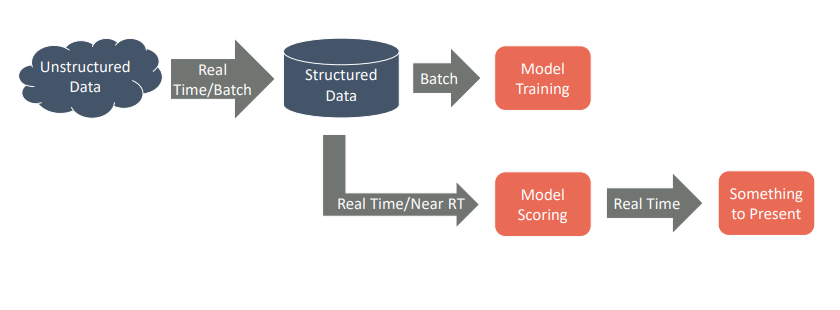
\includegraphics[scale=0.3]{22-a-claassic-big-data-challenge}
\end{center}

\subsubsection{From ETL to ELT}

\begin{center}
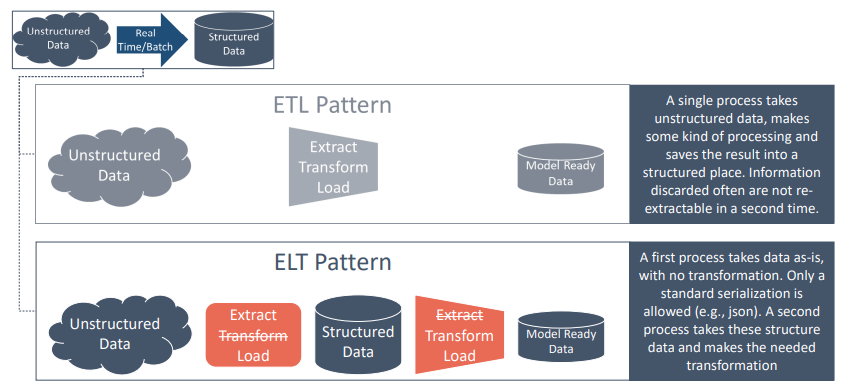
\includegraphics[scale=0.3]{23-from-etl-to-elt}
\end{center}